\documentclass[a4paper,fleqn]{cas-dc}


\usepackage[numbers,sort&compress]{natbib}
\usepackage{prisma-flow-diagram} 
\def\tsc#1{\csdef{#1}{\textsc{\lowercase{#1}}\xspace}}
\tsc{WGM}
\tsc{QE}

\begin{document}
\let\WriteBookmarks\relax
\def\floatpagepagefraction{1}
\def\textpagefraction{.001}

% Short title
\shorttitle{Engineering AI Frameworks for Real-Time Financial Fraud Detection: A Systematic Review}    

% Short author
\shortauthors{D. Amaral and L. Faria}  

% Main title of the paper
\title [mode = title]{Engineering AI Frameworks for Real-Time Financial Fraud Detection: A Systematic Review}  

\tnotemark[1] 
\tnotetext[1]{}
\author[1]{Diogo Amaral}%[<options>]
\cormark[1]
\fnmark[1]
\ead{1160088@isep.ipp.pt}
\ead[url]{}
\credit{Conceptualization, Methodology, Software, Formal analysis, Investigation, Writing - original draft}

\affiliation[1]{organization={Instituto Superior de Engenharia do Porto (ISEP)},
            city={Porto},
            country={Portugal}}

\author[2]{Luiz Faria}

\fnmark[2]
\ead{lef@isep.ipp.pt}

\ead[url]{}
\credit{Supervision, Conceptualization, Writing - review \& editing}
\affiliation[2]{organization={Instituto Superior de Engenharia do Porto (ISEP)},
            city={Porto},
            country={Portugal}}

\cortext[1]{Corresponding author}
\fntext[1]{https://orcid.org/0009-0004-0155-6817}

\begin{abstract}
The rapid expansion of digital payment systems has been accompanied by increasingly sophisticated fraud schemes, posing significant risks to financial stability and consumer confidence. 
This systematic review examines studies published between January 2021 and October 2025 on the use of Machine Learning (ML) in financial fraud detection, focusing particularly on card-based payments, online banking, and real-time transaction monitoring. 
Following the PRISMA 2020 guidelines, evidence was drawn from multiple bibliographic databases to ensure a comprehensive and reproducible synthesis of the field.
The review develops a structured taxonomy that categorises AI techniques into supervised, unsupervised, semi-supervised, deep learning, graph-based, federated, and explainable AI approaches, distinguishing between batch and real-time operational contexts. 
Beyond comparing model performance, it critically discusses methodological practices, evaluation metrics, and deployment challenges, including class imbalance, concept drift, adversarial robustness, and the growing demand for transparent and accountable systems.
The analysis suggests a growing use of advanced architectures such as Transformers and Graph Neural Networks, ensemble strategies, and privacy-preserving techniques like federated learning, alongside an increasing use of model-agnostic explainability tools. 
Drawing on these insights, the review highlights ongoing challenges related to real-world evaluation, cross-institutional data sharing, robust learning under drift, and the lack of standardised benchmarks.
Finally, the review synthesises critical open challenges and delineates a clear frontier for future research, emphasising the need for system-centric evaluation rather than isolated algorithmic improvements.
\end{abstract}


\begin{highlights}
\item Comprehensive PRISMA-compliant systematic review of AI and ML frameworks for financial fraud detection, spanning studies published between January 2021 and October 2025
\item Structured taxonomy categorising contemporary approaches into supervised, unsupervised, deep learning, graph-based, federated, and explainable AI (XAI) across transaction, entity, and network levels
\item Critical analysis of cross-cutting technical challenges, specifically addressing extreme class imbalance, concept drift, adversarial robustness, and the growing demand for regulatory-aligned transparency
\item Identification of an apparent technological shift from classical tree-based ensembles toward advanced architectures such as Transformers, Graph Neural Networks (GNNs), and privacy-preserving Federated Learning
\end{highlights}



% Keywords
\begin{keywords}
Fraud Detection \sep 
Machine Learning \sep
Deep Learning \sep
Explainable AI \sep
Graph Neural Networks \sep
Anomaly Detection \sep
\end{keywords}

\maketitle

% Main text
\section{Introduction}
Financial fraud remains a widespread global challenge, with losses from payment fraud, account takeover, and related crimes estimated to reach trillions of dollars each year \cite{sarna_ai_2025, mill_opportunities_2023}. 
Traditional rule based and scorecard systems, though once effective, increasingly struggle to keep pace with adaptive adversaries who exploit the growing complexity and speed of digital payment \cite{banirostam_analysis_2024, madhavappa_efficient_2025}.
At the same time, the availability of large-scale transactional data and advances in ML have created new opportunities to detect non-linear patterns of fraudulent behaviour, capture temporal and relational dependencies, and adapt dynamically to emerging attack strategies \cite{deng_transformer-based_2025, kumar_revolutionising_2025}. 

Over the past decade, researchers have applied a broad range of ML techniques, from classical models such as logistic regression, decision trees, and random forests, to gradient-boosted ensembles and deep learning architectures like recurrent networks, autoencoders, Transformers, and Graph Neural Networks, across domains including credit card payments, online banking, e-commerce, insurance, and cryptocurrency transactions and financial statement fraud  \cite{bin_sulaiman_review_2022, sarna_ai_2025, hashemi_fraud_2023, wang_temporal_2023, abadlia_enhanced_2025, abdullah_machine_2024, li_uncovering_2024, wei_evaluation_2023, wu_enhanced_2024}.

However, these studies differ greatly in terms of data realism, evaluation protocols, and the extent to which they align with operational constraints such as real-time decision-making, regulatory compliance, and limited computational resources in production environments \cite{chen_deep_2025, ahmed_secure_2024, khan_model-agnostic_2025}. 

There is therefore a pressing need for a systematic assessment that goes beyond algorithmic novelty to evaluate how AI based fraud detection methods perform under realistic deployment conditions.
Several surveys and reviews have summarised fraud detection techniques, typically focusing on specific subdomains (e.g. credit card fraud, anti-money laundering) or classes of algorithms (e.g. traditional classifiers or anomaly detection) \cite{adejoh_adaptive_2025, mousavian_review_2025, cherif_credit_2023, lalit_imbalance_2025}. 
While these earlier reviews have provided valuable overviews of datasets and methods, they also reveal several limitations that reduce their relevance to the contemporary landscape \cite{cherif_credit_2023, bin_sulaiman_review_2022, lim_review_2021}.

Many predate the rapid advances since 2020 in graph-based deep learning, Transformer-style sequence models, federated learning, and user-centric explainable AI \cite{alarfaj_enhancing_2025, deng_transformer-based_2025, khan_model-agnostic_2025}. 
Fraud detection is also frequently framed as a conventional classification or anomaly-detection problem, with limited attention to real-time operational requirements, regulatory expectations, or cross-institutional collaboration \cite{mill_opportunities_2023, awosika_transparency_2024, chhabra_voting_2023}. 
In addition, methodological aspects such as explicit search and inclusion criteria, mitigation of data leakage, treatment of concept drift, assessment of risk of bias, and adversarial robustness are often only briefly addressed\cite{cherif_credit_2023, khan_model-agnostic_2025, hafez_systematic_2025}.

This review is designed to address these gaps through a PRISMA-aligned systematic analysis of AI-driven fraud detection in financial transaction systems, focusing on studies published between 2021 and 2025. 
The scope encompasses card-present and card-not-present payments, online and mobile banking, and closely related transactional settings, while also drawing comparative insights from adjacent domains such as e-commerce and blockchain where detection techniques are transferable to payment fraud scenarios \cite{hafez_systematic_2025}.

The objectives of the review are fourfold. 
The first is to develop a structured and up-to-date taxonomy of machine learning methods for financial fraud detection, covering supervised, unsupervised, semi-supervised, deep, graph-based, federated, and explainable approaches \cite{blaszczynski_auto_2021}. 
The second is to critically evaluate the reported performance of these methods across fraud domains, data modalities, and deployment environments, with particular emphasis on evaluation metrics, class imbalance, and experimental design. 
The third objective is to analyse operational and methodological challenges, including extreme class imbalance, concept drift, adversarial attacks, privacy and data-governance constraints, and the trade-off between accuracy and interpretability. 
The final objective is to synthesize the evidence to identify high-priority research gaps and delineate the essential characteristics required for next-generation, deployment-ready AI fraud detection systems.

To guide this investigation, the review is structured around three research questions:
\begin{itemize}
\item RQ1: What categories of ML methods have been employed for detecting fraud in financial transaction systems since 2021, and how are they deployed across different data types and system architectures?
\item RQ2: How do these methods perform in terms of predictive accuracy, discrimination, and operational utility, and how robust are the reported results to methodological choices such as dataset selection, handling of class imbalance, and prevention of data leakage?
\item RQ3: What methodological, technical and regulatory challenges remain insufficiently addressed, and what future research directions emerge for constructing scalable \cite{mill_opportunities_2023, sarna_ai_2025}, privacy‑preserving, explainable and adversarially robust fraud detection systems?
\end{itemize}
The remainder of this paper is organised as follows. Section 2 describes the systematic review methodology, including protocol registration, information sources, search strategy, eligibility criteria, study selection, data extraction, and quality appraisal. The following sections present a taxonomy of ML methods for fraud detection, report the qualitative and semi‑quantitative synthesis of findings, discuss cross‑cutting challenges and research gaps, and conclude with a discussion of the implications for practice and future research.

\section{Methodology}

This study was conducted as a systematic review of research on ML methods for financial fraud detection, following the PRISMA 2020 guidelines. 
The review protocol was pre-registered in an open repository to enhance transparency and ensure reproducibility. 

This section outlines the methodological framework, covering protocol registration, eligibility criteria, information sources, search strategy, study selection, data extraction, quality appraisal, and synthesis procedures.

\subsection{Protocol and registration}
A detailed review protocol was developed prior to commencing the literature search.
It defined the research objectives and questions, eligibility criteria, databases, search strategies, screening and selection procedures, data extraction schema, quality assessment tools, and synthesis methods. 
Any subsequent amendments, such as refinement of search strings or minor adjustments to inclusion criteria, were recorded and justified in the protocol documentation.

The review followed the PRISMA 2020 checklist, and reporting in both the main text and supplementary materials is mapped to the key PRISMA items. 
This includes transparent documentation of information sources, search strategies, selection decisions, and the assessment of risk of bias.

\subsection{Eligibility criteria}
Eligibility criteria were defined using an adapted PEO (Population–Exposure–Outcome) framework tailored to AI financial fraud detection.

For the Population/Problem, we considered systems and environments involving financial transaction data in domains such as card-based payments (credit, debit, and prepaid cards), online and mobile banking, payment gateways and merchant-acquiring or e-commerce platforms, as well as blockchain-based or cryptocurrency ecosystems whenever the primary objective was the detection of fraudulent or otherwise illicit transactions \cite{alutaibi_blockchain_2025, baabdullah_efficiency_2024}.

The Exposure/Intervention dimension required that studies design, implement, or evaluate Machine Learning methods for fraud detection. Eligible interventions spanned supervised learning, unsupervised and anomaly-detection methods, semi-supervised and weakly supervised approaches, deep learning architectures, graph-based models, and federated or otherwise distributed learning frameworks, including privacy-preserving schemes \cite{baabdullah_efficiency_2024, dang_comprehensive_2024}. 
We also included studies that applied explainable AI techniques specifically to fraud detection models, as well as hybrid and ensemble approaches that combined any of these model families within an integrated fraud detection pipeline.

Regarding Outcomes, studies were required to report at least one quantitative performance metric that is standard in fraud detection practice. 
Acceptable measures included classification metrics such as accuracy, precision, recall, F1-score, specificity, and Matthews correlation coefficient, discrimination metrics such as area under the AUC-ROC and area under the PR-AUC and operational indicators such as false-positive rate at fixed recall, precision at top-k, cost sensitive measures, or latency and throughput statistics for real-time scoring. 
In addition, studies had to provide sufficient methodological detail—covering, at a minimum, the dataset, the train–test split, and the validation procedure, to allow a basic appraisal of internal validity.

Within this PEO structure, we included peer-reviewed journal articles and full conference papers published between 2021 and 2025 that focused on detecting fraudulent or anomalous behaviour in financial transactions, including work on risk or credit scoring only when it explicitly targeted fraudulent default or misreported identity. 
System and framework papers were eligible when AI or ML models formed a core component of the fraud detection pipeline. 
Systematic reviews and meta-analyses of fraud detection methodologies were also included, but solely for contextualisation and cross-validation of our findings rather than as primary evidence on model performance.

We excluded studies that dealt exclusively with non-financial fraud domains such as email spam, generic cyber-intrusion, or social media bot detection without clear transferability to financial transaction fraud. 
We also excluded work on healthcare, insurance, or supply-chain fraud when financial transaction data were not central or the operational context was not comparable to payment systems. 
Theoretical or purely conceptual contributions without empirical evaluation on real or realistically simulated transaction data were not considered, nor were short papers, posters, extended abstracts, editorials, non–peer-reviewed reports, or studies published in languages other than English.

\subsection{Information sources}
To obtain comprehensive coverage of both computer science and financial systems research, several electronic databases and digital libraries were consulted, including Web of Science, Elsevier ScienceDirect, and SpringerLink, making these data sources essential for avoiding any type of bias.

\subsection{Search Strategy}
The core search concepts were Financial fraud and related phenomena, ML techniques and Detection/monitoring focus. Controlled vocabularies (where available) and free‑text terms were combined using Boolean operators and field restrictions.
In Web of Science, the search was conducted using the following query: 

\textbf{("Fraud Detection") And ( "Artificial Intelligence" OR  "Machine Learning") and ("Challenges" or "Techniques")}
including only the Web of Science Categories, Computer Science Theory Methods, Computer Science Information Systems, Engineering Electrical Electronic and Computer Science Artificial Intelligence.

In ScienceDirect and Springer, the search was conducted using the following query: 

\textbf{("Finance" and "Fraud Detection") And ( "Artificial Intelligence" OR  "Machine Learning") and ("Challenges" or "Techniques")}
including only the subject areas of Computer Science and Engineering.

Filters were applied to restrict results to the period 2021–2025, to the English language, and to document types corresponding to peer‑reviewed journal articles and full‑length conference papers. 
All search strategies, including database specific adaptations and any refinements made during scoping, were documented in the PRISMA and are provided in full in the supplementary material to support reproducibility.

\subsection{Selection process}
All retrieved records were exported and managed using Zotero for reference organisation and Rayyan for screening. 
The search process identified 1,124 records across the three databases.
Duplicate records were removed using automated matching (based on title, author, DOI, and publication year), followed by manual verification, removing 24 duplicates in total. 
The selection process proceeded in two stages:

First, two reviewers independently screened titles and abstracts against the eligibility criteria, labelling each record as “included” or “excluded”. This stage resulted in 397 included and 703 excluded papers.

Second, the full texts of the included records were retrieved and reviewed independently by both reviewers. Reasons for exclusion at this stage were carefully recorded (e.g., incorrect domain, absence of AI components, insufficient methodological transparency, or missing quantitative results). Following full-text screening, 99 studies were retained for qualitative and quantitative synthesis, while 298 were excluded.

A PRISMA 2020 (Figure 1) flow diagram summarises the identification, screening, and inclusion stages, providing full counts and exclusion reasons at each step.

\begin{figure}
	\centering
	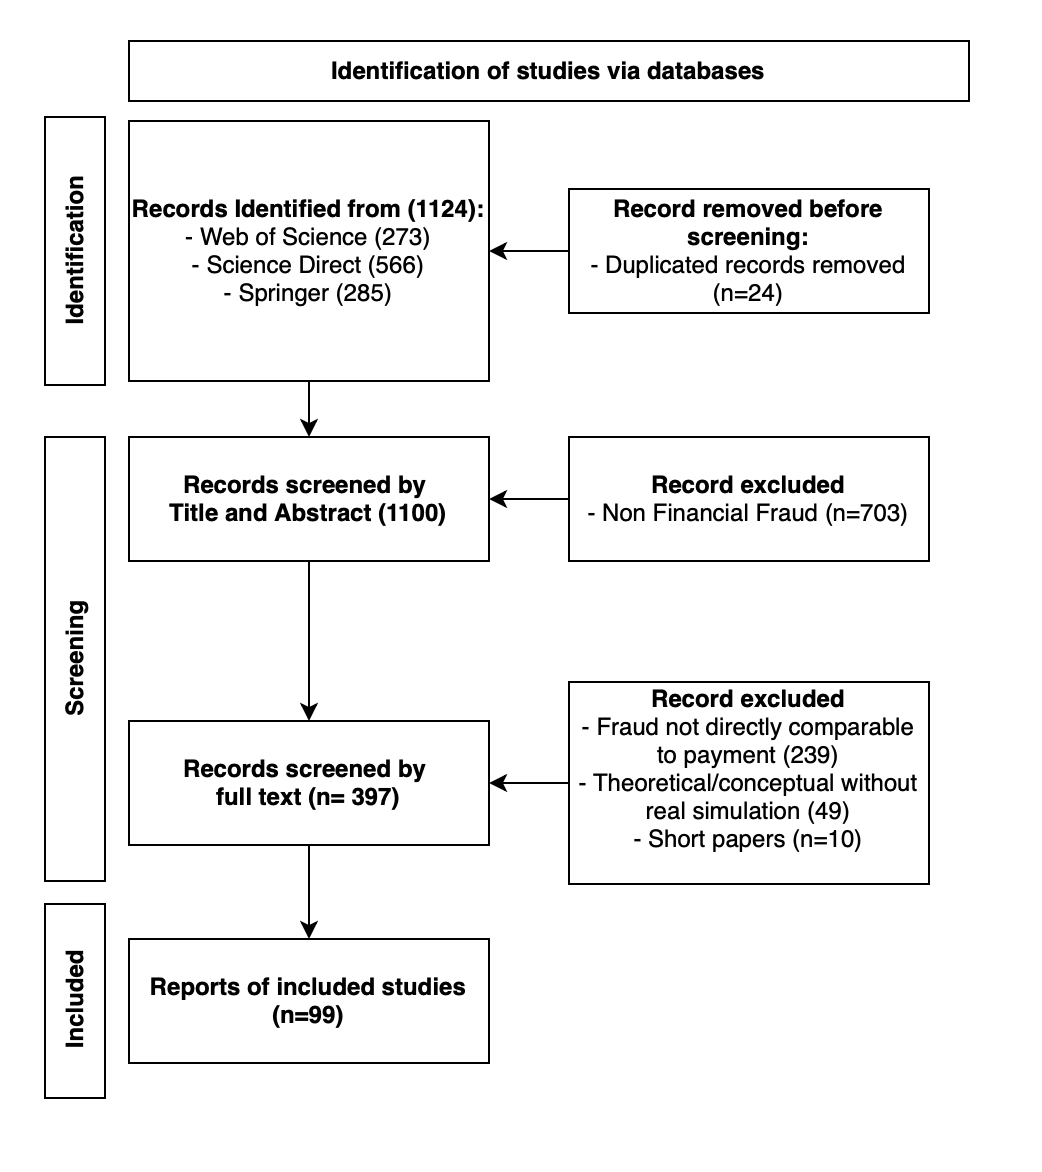
\includegraphics[width=1\columnwidth]{figs/prisma.png}
	\caption{PRISMA 2020 flow diagram}
	\label{FIG:1}
\end{figure}

\subsection{Data extraction}
A standardised data extraction form was developed and piloted on a small subset of the included studies to ensure consistency and clarity. 
The form was designed to capture a comprehensive range of information across several dimensions:

Bibliographic details: Author names, year of publication, publication venue (journal or conference), and, where relevant, the country or region associated with the study.

Fraud domain and context: Type of fraud investigated (e.g. card‑present, card‑not‑present, anti‑money laundering, online banking, e‑commerce, or crypto‑asset transactions), the institutional setting (bank, payment processor, marketplace, etc.), and whether the focus of the study was on detection, prevention, or both.

Data characteristics: Dataset name or source (e.g. public benchmark or proprietary), sample size, number of features, class imbalance ratio, temporal characteristics such as the period covered, and data modality (tabular, sequential, graph‑structured, or multimodal).

Model characteristics: Machine Learning or AI techniques employed (e.g. random forest, XGBoost, LSTM, Transformer, Graph Neural Network, autoencoder, GAN, federated learning framework, or XAI technique). Where applicable, model architecture details and any hybrid or ensemble configurations were also recorded.

Evaluation protocol: Training, validation, and testing procedures; cross‑validation strategies, hold‑out type (temporal or random split), presence of external validation; approach to hyperparameter tuning (e.g. grid search, Bayesian optimisation, or metaheuristics) and any measures implemented to minimise data leakage.

Performance metrics: Reported metrics such as accuracy, precision, recall, F1‑score, AUC‑ROC, PR‑AUC, MCC, and cost‑sensitive or latency‑related measures. 
The primary comparison metric, along with any confidence intervals or statistical tests, was also documented.

Operational and regulatory aspects: Consideration of real‑time constraints, deployment architecture, strategies for managing concept drift, adversarial robustness, privacy preserving measures, and explainability or model transparency approaches.

Authors’ conclusions and limitations: Summary of key findings, reported limitations, and any commentary on generalisability or proposed directions for future research.

The extraction form was refined iteratively as new patterns and reporting styles were encountered, with all modifications recorded in the review protocol to maintain methodological transparency.

\subsection{Quality appraisal and risk of bias assessment}
Given the heterogeneity of ML studies in terms of data, methods, and evaluation practices, a tailored quality assessment instrument was developed by adapting elements from existing tools for diagnostic test accuracy and prediction model studies. 
The instrument included criteria grouped into the following domains:

Data and sampling: representativeness of the dataset with respect to real‑world fraud prevalence and patterns, clarity of inclusion/exclusion criteria for data and handling of missing data.

Study design and evaluation: appropriateness of the train/test split (particularly temporal splits for time‑dependent data), use of external validation, avoidance of data leakage (e.g. preventing leakage of future information, customer‑level splitting), adequacy of hyperparameter tuning and model selection procedures.

Outcome measurement: choice of performance metrics in relation to class imbalance and operational objectives, reporting of multiple complementary metrics (e.g. PR‑AUC alongside AUC‑ROC), provision of uncertainty estimates where possible.

Model complexity and interpretability: consideration of overfitting, regularisation, calibration, and interpretability or explainability where relevant.

Reporting transparency: completeness of methodological description, including model configuration, feature engineering, and computational budget.
 
Each study was assessed independently by two reviewers on these criteria, using a three‑level scale (low, moderate, or high risk of bias/concern) for each domain. 
An overall judgement of study quality was recorded, and any discrepancies were resolved by discussion. Quality assessment results were used to contextualise the synthesis (e.g. by giving more weight to robustly designed studies and highlighting where evidence is based on high‑risk‑of‑bias work).

\subsection{Synthesis methods}
Given the diversity of datasets, model types, and evaluation protocols, a formal meta‑analysis was not anticipated to be feasible for most outcomes. 
Instead, a mixed narrative and semi‑quantitative synthesis approach was adopted:

Studies were grouped by fraud domain, data modality, and primary model family (e.g. tree‑based ensembles, sequence models, graph‑based models, federated approaches).

Within each group, ranges of key performance metrics (such as AUC‑ROC, PR‑AUC, recall at specified false‑positive rates) were summarised, with explicit reference to dataset type (public vs proprietary), class imbalance, and evaluation design.

Where multiple high‑quality studies evaluated comparable methods on the same or closely related datasets, performance comparisons were discussed, with attention to methodological differences.

Cross‑cutting themes (e.g. handling of class imbalance, concept drift, XAI, privacy, adversarial robustness) were synthesised in dedicated sections, drawing on evidence across multiple domains and model families.

Throughout the synthesis, particular care was taken to distinguish between results obtained on idealised benchmark datasets and those derived from production, like or proprietary data, and to highlight where performance claims are potentially inflated by optimistic evaluation protocols or uncontrolled sources of bias.

\section{Taxonomy and Technical Synthesis}
This section develops a structured taxonomy of ML methods for financial fraud detection and synthesises the technical evidence from recent studies. 
The taxonomy is organised along three axes: (1) problem formulation and operational context, (2) data modality and (3) model family. 
Within each class, we highlight typical use‑cases, architectural patterns, and strengths and limitations in production oriented settings.

\subsection{Problem formulation and operational context}
Financial fraud detection systems differ not only in the models they employ, but also in the way the underlying task is framed. 
For clarity, we distinguish three principal levels of analysis and two operational regimes.


\subsubsection{Levels of analysis}
Transaction‑level detection: The most common formulation treats each transaction (card payment, transfer, crypto transfer) as an individual instance to be classified as fraudulent or legitimate \cite{bin_sulaiman_review_2022, cherif_credit_2023, ahmed_secure_2024, adil_optdevnet_2024, karthika_smart_2023, karthikeyan_intelligent_2023, madhavappa_efficient_2025, abdullah_machine_2024, ravindranath_evaluation_2024}. 
Models are trained on tabular or sequential features and optimised for discriminative metrics such as AUC‑ROC, PR‑AUC, F1‑score, or recall at fixed false‑positive rates \cite{almazroi_online_2023, kennedy_synthesizing_2024}. This level underpins most card‑not‑present and online banking fraud systems \cite{almazroi_online_2023, ranganatha_enhancing_2025}.

Account or entity‑level risk scoring: 
Some methods focus on assigning risk scores to accounts, customers, devices, or merchants rather than individual transactions \cite{talaat_precise_2025, wu_heterogeneous_2024, wei_evaluation_2023, wu_enhanced_2024, zhang_multi-view_2025}. 
Here the target can represent propensity for future fraud, susceptibility to takeover, or likelihood of involvement in money‑laundering schemes \cite{talaat_precise_2025}. 
Aggregated behavioural features (e.g. long‑term velocity, diversity of counterparties) and temporal patterns are particularly important \cite{chen_variational_2021}.
Entity-level risk scoring has been applied to anti-money laundering using variational autoencoders \cite{chen_variational_2021} and to bank account monitoring with unsupervised isolation forests and SHAP explanations \cite{karnavou_i_2025}.
Recent work on heterogeneous graph neural networks targets supply chain finance fraud \cite{wu_heterogeneous_2024}, while metagraph-based architectures detect collusion in transaction networks.

Network‑level fraud and collusion detection: Graph‑based approaches frame fraud as a network phenomenon, aiming to detect fraud rings, collusive merchant networks, or money‑laundering chains \cite{wu_heterogeneous_2024}. The objective can be to label nodes (entities), edges (transactions or relationships), or subgraphs as anomalous or suspicious \cite{van_belle_shine_2024, wu_heterogeneous_2024}. This level is increasingly important for high‑value schemes and organised financial crime \cite{li_fedgat-dcnn_2024}.

\subsubsection{Batch versus real‑time regimes}
Batch and near‑real‑time scoring: Many academic studies assume batch processing, with access to complete historical datasets and no hard latency constraints \cite{van_belle_shine_2024, wu_heterogeneous_2024, li_fedgat-dcnn_2024}. 
Outputs are evaluated offline, and models can be retrained periodically \cite{van_belle_shine_2024}. 
Even when studies claim “real‑time” relevance, latency is often reported only indirectly (via algorithmic complexity) rather than measured explicitly \cite{van_belle_shine_2024}.

True real‑time and streaming detection: Production systems in card payments and online banking typically require decisions within tens of milliseconds \cite{alarfaj_enhancing_2025, van_belle_shine_2024}. 
This constrains model complexity, feature computation, and explanation strategies \cite{li_fedgat-dcnn_2024}. 
Only a subset of the surveyed methods is explicitly evaluated under hard latency budgets, and there is a notable gap between offline performance reports and evidence of deployment‑ready architectures \cite{li_fedgat-dcnn_2024, van_belle_shine_2024, plakandaras_credit_2022, sobana_sophisticated_2025}.

The taxonomy presented below maps model families to these problem formulations and operational regimes.

\subsection{Data modalities and feature representations}
Fraud detection pipelines operate on heterogeneous data. 
We distinguish four main modalities, which strongly influence the choice of model architectures.

Static tabular features: Engineered attributes at the transaction or account level (amounts, merchant codes, device and IP attributes, historical spending aggregates) \cite{almazroi_online_2023, alfaiz_enhanced_2022, ravindranath_evaluation_2024, sobana_sophisticated_2025}. 
Classical ML, tree‑based ensembles and feed‑forward neural networks are most common here \cite{almazroi_online_2023, alfaiz_enhanced_2022, zhao_improved_2024}.

Sequential and event‑stream data: Ordered sequences of events (transactions, logins, device changes), sometimes across multiple channels \cite{zioviris_intelligent_2024, alam_intelligent_2023, akour_hybrid_2025, deng_transformer-based_2025, wei_evaluation_2023}. 
Sequence models such as RNNs, LSTMs, GRUs, and Transformers exploit temporal dependencies and contextual patterns in these streams \cite{zioviris_intelligent_2024, akour_hybrid_2025, deng_transformer-based_2025, alam_intelligent_2023}.

Graph‑structured data: Entities (customers, cards, merchants, devices, IPs, wallets) connected via transactions or shared attributes. 
Graph‑based methods, Graph Neural Networks, Graph Attention Networks, and related architectures, leverage relational structure and higher‑order connectivity \cite{boyapati_balancergnn_2025, van_belle_shine_2024, li_fedgat-dcnn_2024}.

Hybrid and multimodal representations: Combinations of tabular, sequential, and graph features, or fusion of transactional data with external signals (e.g. device fingerprinting, behavioural biometrics, blacklists) \cite{wu_heterogeneous_2024, alarfaj_enhancing_2025, ileberi_hybrid_2024, sivasubramanian_predicting_2024, zhang_multi-view_2025}. 
Hybrid architectures often combine separate modules (e.g. GNN + LSTM + gradient‑boosted trees) with ensemble strategies at the scoring layer \cite{wu_heterogeneous_2024, akour_hybrid_2025, ileberi_hybrid_2024, krishnavardhan_intelligent_2024}.

\subsection{Taxonomy of model families}

\subsubsection{Classical supervised learning and tree‑based ensembles}
Logistic regression and linear models remain relevant as baselines and in highly regulated environments \cite{iqbal_time_2024, chhabra_voting_2023, el_barakaz_optimization_2022, plakandaras_credit_2022}. 
Their advantages are simplicity, interpretability, and ease of deployment, but they struggle to capture complex non‑linear interactions and high‑dimensional feature spaces typical of contemporary fraud settings \cite{iqbal_efficient_2025}.

Decision trees and Random Forests offer greater flexibility, handling heterogeneous features and non‑linear relationships with relative robustness \cite{blaszczynski_auto_2021, korkoman_evolutionary_2023}. 
Random Forests appear in many e‑commerce and click‑fraud studies \cite{xie_enhanced_2023}, where they demonstrate competitive performance with moderate tuning effort. 
However, they may underperform more advanced ensembles on highly imbalanced or high‑dimensional problems and can be difficult to calibrate in extreme class imbalance regimes \cite{van_belle_shine_2024}.

Gradient‑boosted trees (notably XGBoost, LightGBM and CatBoost) have become de facto workhorses in tabular fraud data. XGBoost is reported in multiple studies to achieve AUC‑ROC values in the 0.96–0.99 range on both public and proprietary datasets, with strong robustness and built‑in regularisation \cite{alsowail_optimizing_2025, zhao_improved_2024, tayebi_novel_2025, sivasubramanian_predicting_2024}. 
LightGBM typically provides similar discrimination with significantly reduced training times \cite{marazqah_btoush_enhancing_2025, han_enhanced_2025} and lower memory footprint, making it attractive for near‑real‑time scenarios \cite{hashemi_fraud_2023, zhao_improved_2024, ravindranath_evaluation_2024}. 
CatBoost is particularly effective when dealing with high‑cardinality categorical features (e.g. merchant IDs, device IDs), reducing the need for extensive preprocessing \cite{alsowail_optimizing_2025}.

Tree-based ensembles exhibit several strengths, including high predictive performance on engineered tabular features, flexibility in capturing non-linear feature interactions, and mature implementations with good production-deployment support. 
However, they also present limitations, such as susceptibility to overfitting when aggressive resampling or data leakage is present, limited ability to exploit sequential or relational structure unless such patterns are manually encoded as features, and opacity in large models that necessitates post-hoc explainability methods.

\subsubsection{Deep learning for tabular and sequential data}

Feed‑forward deep neural networks (DNNs) are used to model complex feature interactions in tabular data and to ingest mixed feature types. 
Fine‑tuned DNNs can outperform classical models when sufficient labelled data and good regularisation are available, but they often require careful architecture design and significant computational resources \cite{krishnavardhan_intelligent_2024, de_zarza_optimizing_2023}. 
Their black‑box nature raises concerns about interpretability.

Recurrent neural networks (RNNs), LSTMs and GRUs are prevalent in sequential fraud detection tasks where transaction history and behavioural trajectories are crucial \cite{karthikeyan_intelligent_2023, akour_hybrid_2025, zioviris_intelligent_2024, alam_intelligent_2023, sivasubramanian_predicting_2024, sobana_sophisticated_2025, wei_evaluation_2023}. 
Bi‑directional LSTMs and attention‑augmented LSTMs capture both short and long‑range dependencies, improving recall on subtle behavioural shifts such as account takeover or gradual escalation of transaction amounts \cite{sulaiman_credit_2024, hu_hybrid_2025, ranganatha_enhancing_2025}. 
Studies report high classification accuracy and recall, but comparisons against strong tree‑based baselines are sometimes inconclusive, particularly on static tabular datasets.

Transformer‑based architectures have recently been adapted to transaction sequences and multi‑channel event streams \cite{kandi_enhancing_2025}. 
By relying on self‑attention mechanisms, Transformers can model long‑range and cross‑channel dependencies without explicit recurrence and are naturally suited to parallel processing. 
Hybrid graph‑Transformer models aggregate both temporal and topological information, and early evidence suggests meaningful gains in capturing gang fraud patterns. 
However, Transformers introduce challenges in terms of computational cost \cite{ileberi_hybrid_2024}, memory footprint, and the need for careful regularisation, especially under severe class imbalance.

Across deep sequence models, the main benefits are, automatic representation learning from raw or minimally processed sequences, improved recall for rare and complex fraud patterns and flexibility to incorporate attention mechanisms and multi‑head context aggregation.

Key limitations include, Dependence on large, high‑quality labelled datasets, Potential mismatch between offline training regimes and real‑time operational constraints and	Difficulty in providing intuitive explanations without dedicated XAI tools.

\subsubsection{Graph‑based models and network‑centric fraud detection}

Graph‑structured approaches recognise fraud as a relational phenomenon.
Graph Neural Networks (GNNs), including Graph Convolutional Networks (GCNs), GraphSAGE and Graph Attention Networks (GATs), learn node and edge embeddings by aggregating information from local neighbourhoods. 
They are particularly effective at uncovering fraud rings, collusive behaviour and identity‑linking patterns that are otherwise hard to detect.

Architectures such as graph‑augmented recurrent networks and graph self‑attention Transformers combine temporal dynamics with graph convolutions, allowing models to reason jointly about the order of transactions and the connectivity of entities. 
In the studies reviewed, graph-based models often perform well in coordinated-fraud settings, outperforming strong non‑graph baselines in metrics such as recall at low false‑positive rates and precision within high‑risk segments, especially in scenarios involving coordinated attacks.

Despite their promise, graph‑based models face important challenges like construction and maintenance of large, dynamic transaction graphs at scale, handling of evolving graph structure under concept drift and changing user populations, integration with real‑time scoring pipelines, where subgraph extraction and message passing must meet stringent latency requirements, and Interpretability, given that learned relational patterns can be opaque without specialised explanation mechanisms.


\subsubsection{Unsupervised and anomaly‑detection methods}

Unlabelled or weakly labelled data are ubiquitous in fraud detection, motivating the use of unsupervised methods.

Autoencoders and variational autoencoders (VAEs) learn to reconstruct normal behaviour and flag instances with high reconstruction error as anomalies \cite{cakir_enhanced_2024, ouedraogo_data-driven_2021, kennedy_iterative_2023}. 
They are appealing when labels are scarce or delayed and have demonstrated practical utility in monitoring production streams and generating candidate alerts. 
VAEs introduce a probabilistic latent space, enabling more nuanced anomaly scoring, but require careful calibration of thresholds to achieve acceptable alert volumes \cite{kennedy_synthesizing_2024}.

One‑class methods, including One‑Class SVMs and Isolation Forests, offer simpler alternatives for anomaly detection. Isolation Forests \cite{karnavou_i_2025}, in particular, are reported to achieve high accuracy and reasonable computational efficiency, making them suitable for streaming environments with moderate dimensionality. 
Their performance, however, can degrade when normal behaviour is highly heterogeneous or concept drift is pronounced.

Hybrid unsupervised frameworks combine autoencoders, self‑organising maps and restricted Boltzmann machines with adaptive thresholds \cite{yadav_unsupervised_2022}. 
These approaches attempt to dynamically adjust to evolving behaviour, but can be complex to tune and evaluate, particularly when feedback labels are sparse \cite{kennedy_iterative_2023}
Dual-generator GAN architectures (Duo-GAN) further extend this direction by producing more diverse synthetic minority samples than single-generator approaches, yielding measurable improvements in F1-score under extreme class imbalance in financial transaction data \cite{ferreira_when_2021, zhang_multi-view_2025, zhi_research_2025}.

\subsubsection{Metaheuristic optimisation and swarm intelligence}
Metaheuristic algorithms inspired by natural processes, such as genetic algorithms, Particle Swarm Optimisation, differential evolution and more recent bio‑inspired optimisers, play two main roles \cite{abadlia_enhanced_2025, korkoman_evolutionary_2023}:

Firstly, feature selection, identifying compact subsets of informative features, which can reduce computational burden and improve model generalisation \cite{zhi_research_2025}.
Genetic algorithms applied to feature selection across standard classifiers, including decision trees, random forests, and neural networks, have demonstrated consistent reductions in dimensionality while maintaining competitive detection performance on credit card fraud benchmarks \cite{ileberi_machine_2022, krishnavardhan_intelligent_2024, sobana_sophisticated_2025, wei_evaluation_2023, yadav_unsupervised_2022}.

Secondly, Hyperparameter optimisation, tuning complex models (e.g. XGBoost, deep networks) when the search space is too large or non‑convex for manual tuning \cite{hu_hybrid_2025, sulaiman_credit_2024, wu_enhanced_2024, yadav_unsupervised_2022}.

These methods often deliver high reported accuracy with substantially reduced feature sets, but the additional layer of optimisation can obscure reproducibility and make it harder to attribute performance gains to the underlying model versus the optimisation procedure. Furthermore, few studies assess the stability of selected feature sets across time or across institutions \cite{sobana_sophisticated_2025}.

\subsubsection{Federated and privacy‑preserving learning}
Federated learning frameworks address data privacy and governance constraints by enabling collaborative model training across institutions without sharing raw data \cite{awosika_transparency_2024, zhang_optimization_2025}. 
Architectures combining federated training with graph attention and convolutional layers illustrate how cross‑institutional fraud patterns can be learned in a privacy‑preserving way, achieving strong AUC‑ROC performance on multi‑party datasets \cite{li_fedgat-dcnn_2024}.

Key advantages of federated approaches include alignment with regulatory and privacy requirements that restrict centralised pooling of transaction data and Potential to leverage diverse fraud patterns across multiple institutions, improving generalisation \cite{awosika_transparency_2024}.

However, these benefits come with challenges as Handling non‑IID data distributions and institutional heterogeneity, Communication overhead and convergence issues in federated optimisation, Security risks such as model inversion or poisoning attacks targeting the shared model parameters \cite{baabdullah_efficiency_2024, ahmed_secure_2024, dang_comprehensive_2024}.

\subsubsection{Explainable AI (XAI) and human‑centred frameworks}
Explainability is a cross‑cutting concern rather than a separate model family. 
Tree‑based ensembles and deep models are increasingly coupled with post‑hoc explanation techniques such as SHAP and LIME, as well as with user‑centred explanation frameworks tailored to fraud analysts and compliance officers \cite{damanik_advanced_2025, ghosh_novel_2025, talaat_precise_2025}.
Two broad patterns emerge:

Local explanations: justifying individual alerts (e.g. why a specific transaction was scored as high risk), which supports case investigation and appeals processes.

Global explanations: summarising model logic (e.g. which features drive fraud predictions overall), which is important for model governance, documentation and regulatory audits \cite{cerneviciene_explainable_2024, iqbal_efficient_2025}.
Recent work has begun to explore the interaction between class imbalance countermeasures (resampling, synthetic data generation, cost‑sensitive learning) and the stability of explanations, suggesting that some approaches can significantly distort \cite{damanik_advanced_2025}. 
This underscores the need to consider explainability when designing training and resampling pipelines, not only when applying XAI methods post‑hoc.

\subsection{Cross‑cutting technical themes}
Across model families and data modalities, several technical issues recur.

Class imbalance: Fraud datasets are typically highly skewed \cite{kennedy_synthesizing_2024}. 
Techniques such as SMOTE variants, GAN‑based oversampling, hybrid resampling (e.g. SMOTE‑ENN), cost‑sensitive learning, focal loss and intelligent undersampling are widely used \cite{el-naby_efficient_2023, ni_fraud_2024, zhao_improved_2024, aruleba_enhanced_2025}. 
Emerging evidence indicates trade‑offs between predictive gains and interpretability, with some resampling strategies destabilising feature importance \cite{huang_imbalanced_2024}.
Kolmogorov–Arnold Networks (KANs) combined with GAN-based dynamic oversampling and SHAP-based post-hoc explanations have also been shown to improve minority-class recall while preserving feature attribution stability \cite{akouhar_dynamic_2025}.

Concept drift: Fraud patterns evolve in response to detection mechanisms and external factors. While many studies acknowledge drift, fewer implement explicit drift detection, online learning or periodic retraining protocols \cite{iqbal_time_2024}. Sequence and graph models offer some robustness by capturing more general behavioural patterns, but systematic evaluations of long‑term robustness remain scarce \cite{zioviris_intelligent_2024}.

Adversarial robustness and security: ML‑based fraud systems are themselves targets of adversarial attacks, including data poisoning and evasion \cite{baabdullah_efficiency_2024}. 
A small but growing body of work investigates adversarial training and robust optimisation in this context, yet adversarial robustness is far from a standard evaluation dimension \cite{lusito_solving_2024}.

Evaluation metrics and operational alignment: Accuracy and AUC‑ROC dominate reported metrics, even though they can be misleading under extreme class imbalance. More informative metrics, PR‑AUC, precision at top‑k, cost‑based measures, and recall at fixed alert volumes, are used less consistently. Calibration, latency and resource usage are rarely reported, despite their central importance in real‑time payment systems.

Data leakage and experimental validity: Several threat patterns to validity recur: temporal leakage (using future information in training), customer‑level leakage (splitting transactions from the same customer across train and test), and tuning on test data. High headline performance on public benchmarks must therefore be interpreted cautiously unless evaluation protocols are clearly documented.

\subsection{Summary of the taxonomy}
The taxonomy developed in this chapter positions AI methods for financial fraud detection within a three‑dimensional space defined by problem level (transaction, entity, network), data modality (tabular, sequential, graph, multimodal), and model family (from classical ensembles to deep, graph‑based, federated and explainable architectures). 
This structured view reveals clear trends: tree‑based ensembles and deep sequence models dominate transaction‑level detection; graph‑based and federated models are emerging for network‑level and cross‑institutional fraud; and XAI increasingly acts as a necessary layer around complex models to meet operational and regulatory requirements. 
Subsequent sections build on this taxonomy to compare performance across domains and analyse methodological quality.

\section{Synthesis of Findings}
This section synthesises the evidence across domains, metrics and model families, combining numerical performance ranges with a critical, qualitative assessment of how these results should be interpreted. 
The synthesis is structured by (i) fraud domain, (ii) evaluation metrics and (iii) temporal and methodological trends.

\subsection{Performance by fraud domain and model family}
\subsubsection{Credit card and retail payments}
Credit card fraud detection is the most extensively studied domain in the corpus, with numerous works using public datasets (e.g. European cardholder data) and proprietary transaction streams. 
Across these studies, several patterns emerge:

Tree‑based ensembles: XGBoost, LightGBM and CatBoost frequently achieve AUC‑ROC values between approximately 0.96 and 0.99 on credit card datasets, with reported accuracies in the 96–99.8\% range under various resampling and optimisation regimes \cite{ileberi_hybrid_2024}. 
LightGBM often matches XGBoost’s discrimination while reducing training time by factors of around 3–4, and CatBoost has reached very high accuracy values in some comparative studies, particularly where categorical features dominate \cite{hashemi_fraud_2023}.

Deep learning on tabular and sequential data: Dilated convolutional neural networks (DCNNs) trained on credit card data report accuracies around 97–97.4\%, outperforming baseline CNNs by several percentage points \cite{karthika_smart_2023}. 
LSTM and GRU based models show accuracy in the 97–99\% range on benchmark datasets, with some architectures using focal loss achieving particularly high precision on the minority class \cite{krishnavardhan_intelligent_2024}. 
Event‑based deep networks such as OptDevNet report accuracies around 95–96\% while claiming enhanced robustness across different transaction patterns.

Hybrid and stacking ensembles: Stacking frameworks that combine multiple base learners (e.g. random forest, SVM, KNN, XGBoost, CatBoost, logistic regression) typically report F1‑scores between approximately 0.88 and 0.92, with AUC‑ROC values close to 0.99 on highly imbalanced credit card datasets \cite{leevy_threshold_2023, breskuviene_categorical_2023, khalid_enhancing_2024}. 
When resampling strategies such as K‑means SMOTE‑ENN are integrated, AUPRC values can reach around 0.96, indicating strong performance in the high‑precision operating region.

Generative models and oversampling: Generative approaches using VAEs, GANs and hybrid AE‑GAN architectures for synthetic fraud generation often report improvements in minority‑class recall and F1 relative to classical oversampling methods (e.g. SMOTE, ADASYN), while maintaining or improving overall accuracy \cite{chen_variational_2021, ferreira_when_2021, zhi_research_2025}. 
However, the extent of these gains varies considerably across datasets and evaluation protocols, and few studies systematically assess the impact on calibration or out‑of‑sample robustness \cite{tayebi_generative_2025, ferreira_when_2021, zhang_multi-view_2025, zhi_research_2025}.

Overall, credit card fraud studies tend to report very high headline performance figures (accuracy > 99\%, AUC‑ROC near 1.0) on public benchmarks, but these results are often obtained under favourable conditions (e.g. random splits, limited assessment of drift), which may overstate real‑world performance.

\subsubsection{Online payments and e‑commerce}
In e‑commerce and online payment contexts, models must contend with richer behavioural features and stricter latency constraints.

Random forests and classical ensembles are frequently reported as strong baselines for click‑fraud and behavioural anomaly detection tasks, especially when combined with carefully engineered features (e.g. session‑level statistics, device/browser fingerprints).

Studies targeting real‑time online payment streams increasingly explore hybrid architectures that embed CNN or ResNeXt‑style modules for feature extraction before passing into GRU or other sequence classifiers, with reported gains in accuracy and F1 of 10–18 percentage points over simpler baselines.

While overall accuracy and AUC‑ROC remain high in these settings, authors often highlight the importance of achieving acceptable latency; however, explicit latency measurements and throughput benchmarks are rarely present.

\begin{table}[htbp]
\centering
\caption{Key Approaches: Credit Card Fraud Detection}
\label{tab:credit-card-approaches}
\footnotesize
\begin{tabular}{p{1.7cm} p{2.8cm} p{3.8cm}}
\toprule
\textbf{Category} & \textbf{Key Models} & \textbf{Strengths} \\
\midrule
Tree-based & XGBoost, LightGBM, CatBoost & LightGBM 3--4x faster; categoricals \cite{el_barakaz_optimization_2022, zhao_improved_2024}\\
Deep learning & DCNN, LSTM/GRU, OptDevNet & Focal loss minority; sequential \cite{karthika_smart_2023, femila_roseline_autonomous_2022} \\
Hybrid/stacking & RF, SVM, KNN, XGBoost, CatBoost, LR & K-SMOTE-ENN; robust \cite{talukder_integrated_2024, talukder_securing_2024} \\
Generative & VAEs, GANs, AE-GAN & Recall/F1 vs SMOTE/ADASYN  \cite{tayebi_generative_2025, cakir_enhanced_2024} \\
\bottomrule
\end{tabular}
\end{table}

Blockchain analytics and cryptocurrency transaction fraud form a smaller but rapidly growing subset of the literature.

Hybrid transactional models that combine SVM, KNN and random forest in bespoke ensemble frameworks report detection accuracies above 99\% on curated datasets of blockchain transactions \cite{alutaibi_blockchain_2025}.

These works commonly focus on classification metrics and AUC‑ROC; few provide PR‑AUC, cost‑sensitive measures, or detailed analysis of how models perform under shifting transaction patterns or adversarial manipulation.

\subsubsection{Anti‑money laundering and banking fraud}
Banking fraud detection beyond card transactions, including anti‑money laundering (AML), often involves more complex entity networks and temporal dependencies.

Graph‑based models such as MetaFraud‑GNN, evaluated on transaction networks and related benchmarks (e.g. YelpChi, Amazon, Elliptic), show improvements in F1‑macro, AUC and geometric mean on the order of several percentage points over competitive baselines.

Federated graph architectures like FedGAT‑DCNN, tested on multi‑institution datasets, achieve AUC‑ROC values of approximately 0.97 and 0.999 on two credit card datasets, highlighting the potential of privacy‑preserving, cross institution learning.

AML‑oriented studies underline the importance of balancing detection performance with false positive rates and resource constraints in investigations, yet operational metrics (e.g. alert volume per investigator) are rarely quantified \cite{wu_enhanced_2024}.

\begin{table*}[htbp]
\centering
\caption{Performance summary of top-performing models by fraud domain (2021--2025)}
\label{tab:synthesis-performance}
\smallskip
\begin{tabular}{lcccc}
\toprule
\textbf{Domain} & \textbf{Top Models} & \textbf{Avg AUC-ROC} & \textbf{Main Datasets} & \textbf{References} \\
\midrule
Credit Card & XGBoost/LightGBM & 0.96--0.99 & European/Kaggle & \cite{alsowail_optimizing_2025, zhao_improved_2024} \\
Blockchain & GNN/Federated & 0.97--0.99 & Elliptic/Ethereum & \cite{baabdullah_efficiency_2024} \\
Online Banking & CNN-LSTM & 0.95--0.98 & European (Kaggle-like)/Taiwan  & \cite{ileberi_hybrid_2024} \\
\bottomrule
\end{tabular}
\smallskip
\noindent \footnotesize 
\end{table*}

\subsection{Evaluation metrics: usage patterns and limitations}

Across domains, classification and discrimination metrics are widely reported, but their usage is uneven with respect to the realities of extreme class imbalance.

Accuracy is almost universally reported and often extremely high (> 99\%) in credit card and blockchain studies. Given the low base rate of fraud, these figures can be achieved even by models with poor sensitivity, so accuracy alone is a weak indicator of practical utility \cite{plakandaras_credit_2022}.

Precision, recall and F1‑score are common, particularly in credit card fraud work, where minority‑class performance is emphasised. High F1 values (0.8–0.9+) are regularly reported for advanced ensembles and deep models, though recall at very low false‑positive rates, which is more aligned with operational use, is seldom analysed explicitly.

AUC‑ROC is the most frequently used discrimination metric, with values often in the 0.95–1.0 range for ensembles and deep architectures. However, under extreme imbalance, AUC‑ROC can obscure differences in performance in the region of the ROC curve most relevant to deployment (e.g. very low FPR).

PR‑AUC (AUPRC) appears more regularly in some recent credit card studies, where authors explicitly acknowledge that PR‑AUC better reflects the trade‑off between precision and recall in highly imbalanced settings. 
Nonetheless, PR‑AUC is still under‑reported relative to AUC‑ROC \cite{kennedy_synthesizing_2024}.

MCC and cost‑based metrics are used in a minority of works. Where reported, MCC tends to correlate with F1 and AUC‑ROC but offers a more balanced view under skewed class distributions. Cost‑sensitive evaluations, which assign different weights to false positives and false negatives based on economic impact, are rarely implemented, despite their obvious relevance to financial institutions.

Latency and throughput metrics are largely absent, even in papers that claim real‑time or near‑real‑time operation. A few studies discuss computational efficiency qualitatively (e.g. speed‑ups of LightGBM relative to other boosting frameworks), but comprehensive runtime benchmarks are uncommon.

In summary, while standard ML metrics indicate strong discriminative performance for many models, there is a systematic gap between reported metrics and the operational performance indicators that matter in real‑world fraud systems.

\subsection{Imbalance handling and its impact on performance}
Strategies for handling severe class imbalance are ubiquitous and have a measurable impact on both performance and interpretability.

Resampling techniques: Oversampling (including SMOTE and its variants), undersampling, and hybrid methods such as SMOTE‑ENN and K‑means SMOTE‑ENN are widely employed \cite{lalit_imbalance_2025, li_uncovering_2024, ranganatha_enhancing_2025, ravindranath_evaluation_2024, de_zarza_optimizing_2023}. 
These methods typically improve recall and F1 for the minority class and can contribute to very high AUC‑ROC and AUPRC values, but some studies report increased noise and overfitting when synthetic examples are not carefully controlled \cite{al_balawi_credit-card_2023}. 

Cost‑sensitive learning and class weighting: Adjusting loss functions or class weights to emphasise the minority class often yields comparable performance gains to resampling, with less distortion of the underlying data distribution. Recent work examining the interaction of imbalance countermeasures with XAI suggests that cost‑sensitive approaches and feature selection better preserve the stability of feature attributions than aggressive resampling.

Generative models: VAEs, GANs and hybrid generative architectures provide an alternative route to synthetic minority examples. Empirical results indicate that, in some settings, generative oversampling produces more realistic minority instances and yields improved detection performance relative to classical oversampling methods \cite{de_zarza_optimizing_2023}. 
However, training instability and the risk of mode collapse introduce practical challenges, and comparative studies are still relatively few.

\subsection{Temporal and methodological trends}
The 2021–2025 window shows clear shifts in both the technical focus and methodological maturity of AI‑driven fraud detection.

From classical ML to deep and graph‑based models: Earlier work within this period still relies heavily on tree‑based ensembles and classical classifiers for credit card and banking fraud. Over time, there is a marked increase in the use of deep architectures, CNNs, LSTMs, GRUs and, more recently, Transformer‑based models for sequential and time‑series data, as well as GNNs and metagraph‑based architectures for network‑level fraud detection.

Emergence of federated and privacy‑preserving learning: Federated learning models, including those combining GATs and dilated convolutions, appear from around 2023 onwards and gain prominence in 2024–2025, reflecting growing concerns about data privacy and cross‑institution collaboration. These models demonstrate competitive or superior AUC‑ROC to non‑federated baselines when evaluated on federated setups.

Growing attention to explainability and regulation: Explainable AI transitions from a peripheral topic to a central theme, with surveys and research agendas explicitly focused on XAI for credit card. Empirical studies comparing XAI methods and exploring trade‑offs between resampling, performance and interpretability become more common towards the end of the review period.

Systematic reviews and meta‑surveys: Several systematic or quasi‑systematic reviews appear in 2024–2025, focusing on credit card fraud and AI‑enhanced techniques more broadly. These works indicate increasing methodological awareness but still often rely on narrative synthesis, with limited quantitative aggregation.

Methodological improvements and persistent gaps: Over time, more studies begin to report a broader set of metrics (including PR‑AUC), use more sophisticated resampling strategies, and acknowledge concept drift and adversarial threats. Nonetheless, comprehensive evaluation under drift, cross‑dataset validation, and robust assessment of adversarial robustness remain rare.

\subsection{Synthesis across domains and models}

Taken together, the quantitative and qualitative evidence support several overarching conclusions:

Tree‑based ensembles and deep sequence models deliver consistently strong discrimination on tabular and sequential transaction data. In contrast, graph‑based and federated models offer incremental gains in network‑level and cross‑institutional settings.

High headline metrics (accuracy, AUC‑ROC) are common, particularly on public credit card datasets, but are often achieved under evaluation regimes that may not reflect real‑world conditions, especially with respect to temporal splits, drift, and deployment constraints.

Imbalance handling and choice of evaluation metrics materially affect reported performance, complicating direct comparison across studies and highlighting the need for standardised benchmarking practices.

Recent years show a clear shift towards architectures that integrate representation learning (deep and graph models), privacy preservation (federated learning), and explainability (XAI), but the field has not yet converged on best practices for combining these elements in production systems.

These observations motivate the detailed cross-cutting analysis of challenges presented in the following section.


\section{Cross-Cutting Challenges}
AI‑driven fraud detection operates at the intersection of statistical learning, adversarial behaviour, regulatory pressure and operational constraints. 
Across domains and model families, several cross‑cutting challenges repeatedly emerge: extreme class imbalance, concept drift, adversarial manipulation, explainability and governance, and privacy‑preserving learning at scale. 
This chapter synthesises these themes and highlights their interactions.

\subsection{Extreme class imbalance}

Fraud detection is an archetypal rare‑event problem: genuine transactions outnumber fraudulent ones by several orders of magnitude. 
This imbalance affects model training, evaluation, interpretability and deployment \cite{lalit_imbalance_2025}.

Learning under rarity: Standard classifiers tend to be dominated by the majority class, leading to high accuracy but poor fraud recall. 
Oversampling (e.g. SMOTE, SMOTE‑ENN), undersampling, and hybrid strategies are widely used to rebalance the training data, while cost‑sensitive learning and focal loss reweight the objective function to emphasise minority cases. 
Generative models based on VAEs and GANs provide synthetic fraudulent samples that can further improve minority‑class learning \cite{hu_hybrid_2025}.
Regularised GAN architectures (R-GAN) integrating SHAP-guided feature weighting have been shown to generate higher-fidelity anomaly samples, improving detection performance while maintaining explainability under severe class imbalance \cite{lee_advanced_2025}.

Metric selection and evaluation bias: High overall accuracy and AUC‑ROC can mask poor performance on fraudulent instances \cite{sivasubramanian_predicting_2024}. 
Precision, recall, F1‑score and PR‑AUC are more informative in highly skewed settings, yet are still under‑reported in parts of the literature. 
Moreover, differences in imbalance ratios, resampling strategies and metric choice across studies reduce the comparability of reported results.

Impact on interpretability: Recent work shows that certain imbalance countermeasures—particularly aggressive resampling—can distort feature importance and destabilise explanations produced by XAI methods \cite{lalit_imbalance_2025}. 
Cost‑sensitive learning and careful feature selection appear to preserve interpretability better than heavy synthetic oversampling, but systematic evidence remains limited.

Addressing imbalance therefore requires a joint design of sampling strategy, loss function and evaluation metrics, as well as explicit consideration of how these choices influence downstream explanations.

\subsection{Concept drift and non‑stationarity}
Fraud patterns evolve over time as attackers adapt to detection mechanisms, payment products change and customer behaviour shifts. 
This concept drift challenges the assumption that training and deployment data are drawn from the same distribution.

Types of drift: Fraud drift can be gradual (e.g. evolving card‑not‑present tactics), abrupt (e.g. new scam campaigns) or recurring (e.g. seasonal fraud patterns). 
Structural drift in user populations, transaction channels and regulatory frameworks compounds these effects

Limitations of static evaluation: Many studies rely on random or stratified splits and do not enforce temporal separation between training and test sets, which can lead to optimistic estimates of performance and conceal degradation over time. 
Few works report longitudinal experiments or simulate online operation where data arrive sequentially.

Adaptation mechanisms: Proposed solutions include periodic retraining, sliding windows, online learning algorithms, and models designed to capture more stable behavioural representations (e.g. graph‑based embeddings and sequence models). 
However, systematic evaluations of retraining schedules, drift detection methods and their impact on operational metrics are rare.

Interaction with imbalance and labelling delay: Drift is particularly problematic when combined with severe imbalance and delayed labels: fraudulent transactions may only be confirmed after chargebacks or investigations, making timely adaptation challenging. 
This reinforces the importance of semi‑supervised and unsupervised approaches that can detect emerging anomalies without immediate labels.

Robust fraud detection requires moving beyond single snapshot evaluations towards explicit modelling and monitoring of drift, with metrics that capture both short‑term and long‑term robustness \cite{wu_enhanced_2024}.

\subsection{Adversarial attacks and model security}
ML‑based fraud systems are themselves targets of manipulation. 
Attackers can attempt to evade detection, poison training data, or exploit model updates.

Evasion and probing attacks: Fraudsters can adapt transaction patterns to gradually approach decision boundaries, exploit loopholes in feature engineering, or manipulate input fields to mimic legitimate behaviour \cite{ranganatha_enhancing_2025, sivasubramanian_predicting_2024}. 
Few studies explicitly model this adversarial adaptation; most focus on average‑case performance rather than worst‑case behaviour.

Data poisoning and contamination: Poisoning attacks involve injecting crafted fraudulent or “camouflaged” transactions into training data to bias models, reduce sensitivity to attack types, or cause targeted misclassifications. 
Some recent work demonstrates that adversarially generated fraud examples can be used in training to improve robustness, but systematic frameworks for adversarial training in fraud contexts are still emerging.

Security of federated and distributed learning: Federated learning introduces new attack surfaces: malicious participants can contribute poisoned model updates, infer information about others via gradient analysis, or attempt model inversion attacks to extract sensitive details. 
Robust aggregation, anomaly detection on updates, and secure protocols are necessary but not yet standard practice in fraud applications \cite{ranganatha_enhancing_2025}. 

Lack of adversarial evaluation standards: There is no widely adopted benchmark for adversarial robustness in fraud detection. 
Most studies do not report robustness metrics, and those that do often use bespoke threat models, hindering comparison.

Integrating adversarial thinking into model design, training and evaluation is essential if AI‑based fraud systems are to remain resilient against adaptive attackers.

\subsection{Explainable AI and governance}
Explainability is not optional in financial fraud detection: regulators, customers and internal stakeholders demand transparent, auditable decision processes.

Regulatory and organisational drivers: Regulatory frameworks emphasise fairness, accountability and the right to explanation, particularly when automated decisions affect access to financial services. 
In parallel, fraud operations teams require understandable alerts to triage cases efficiently and to justify interventions to customers and auditors.

Local versus global explanations: Local explanation methods (e.g. SHAP, LIME) are used to justify individual alerts by highlighting influential features for specific transactions or accounts.
Global explanations and model summaries provide higher‑level insight into feature importance and decision logic, supporting governance and model risk management.

Tensions with complex models and resampling: Deep models, GNNs and hybrid ensembles offer high discriminative power but are inherently opaque. 
Post‑hoc explanations can be unstable under changes in data distribution, resampling strategy or feature engineering. 
Experimental evidence suggests that some countermeasures for imbalance degrade explanation quality, highlighting a trade‑off between raw accuracy and interpretability.

User‑centred XAI frameworks: Recent contributions propose user‑centred explanation systems that tailor explanations to different stakeholder groups (fraud analysts, data scientists, compliance officers), combining local and global views and integrating them into case management interfaces. 
These approaches show promise but are still in early stages, and their impact on investigation efficiency and trust is not yet well quantified.

Achieving trustworthy AI for fraud detection thus requires the co‑design of models, handling of imbalances, and explanation strategies, calibrated against regulatory and human‑factors constraints rather than pure predictive performance.

\subsection{Privacy‑preserving and federated learning}
Fraud patterns often span multiple institutions, yet transaction data are highly sensitive and subject to stringent privacy and banking secrecy requirements. 
Federated and privacy‑preserving learning aim to reconcile these tensions.

Cross‑institution collaboration: Federated learning allows multiple banks or payment processors to jointly train models without sharing raw data, potentially capturing cross‑institution fraud schemes that are invisible at the single‑institution level. 
Architectures such as FedGAT‑DCNN show that it is technically feasible to integrate GNNs and dilated convolutions into federated pipelines while achieving strong AUC‑ROC.

Heterogeneity and non‑IID data: Institutions differ in customer base, product mix and data quality, leading to non‑IID distributions across participants. 
This can slow convergence, bias models towards dominant institutions, or degrade performance for smaller participants. 
Few studies propose systematic solutions (e.g. personalised federated models, cluster‑based federated learning) in the fraud context.

Privacy, security and compliance: While federated learning mitigates raw data sharing, model updates themselves may leak information. 
Differential privacy, secure aggregation and robust aggregation are candidate safeguards, but integrating them into high‑performance fraud models remains an open research area. Moreover, regulatory acceptance of such architectures is still evolving.

Operational complexity: Deploying federated systems requires coordination of infrastructure, governance and incentives across institutions. 
Most current work remains at a proof‑of‑concept level; real‑world deployments and long‑term evaluations are rare.

Federated and privacy‑preserving learning are therefore both an opportunity and a challenge: they promise richer, more generalisable models but require advances in optimisation, security, governance and regulation.

\subsection{Interactions and open issues}
These cross‑cutting challenges do not occur in isolation; they interact in ways that complicate model design and evaluation.

Imbalance, drift and adversarial adaptation jointly shape the minority‑class behaviour that models must capture, yet most studies address them separately.

Efforts to improve performance under imbalance (e.g. aggressive resampling) can undermine explainability, which is a regulatory requirement.

Federated learning introduces new dimensions of drift (institutional turnover, asynchronous updates) and adversarial risk (poisoned clients), while also constraining the ability to inspect raw data for bias and leakage.

Future work must therefore treat these aspects as components of a unified system design problem rather than as independent technical sub-tasks.

\section{Discussion}
The evidence assembled in this review paints a nuanced picture: 
technically, AI‑driven methods for financial fraud detection are mature and diverse, yet their evaluation and deployment practices often lag behind the complexity and criticality of real‑world environments. 
This chapter discusses the broader significance of the findings and draws out implications for practitioners and regulators.

\subsection{Reconciling headline performance with real‑world constraints}

Across domains, many studies report near‑perfect accuracy and AUC‑ROC values on benchmark datasets, particularly for credit card fraud and blockchain transaction analysis. 
Tree‑based ensembles, deep sequence models and graph‑based architectures consistently outperform simpler baselines under controlled conditions. 
However, these results must be interpreted against several limitations:

Evaluation regimes are often optimistic. 
Random or stratified splits, absence of temporal validation and limited discussion of concept drift suggest that reported performance may not generalise to evolving production environments.

Operational metrics are under‑reported. 
Latency, throughput, alert volumes and investigation capacity—central to deployment decisions—rarely appear in empirical evaluations.  

Adversarial behaviour is largely ignored in evaluation. 
While some works explore adversarial training, systematic robustness testing against targeted evasion or poisoning is still the exception.

The implication for practice is that institutions should treat headline metrics on public datasets as upper bounds rather than guarantees, and should prioritise internal validation with realistic data splits, drift evaluation and stress testing.

\subsection{Trade‑offs between complexity, robustness and interpretability}

The taxonomy and synthesis chapters show a clear trend towards more complex models: 
deep architectures, GNNs, Transformer‑based networks, hybrid ensembles and federated frameworks. 
These models can capture subtle behavioural and relational patterns but introduce trade‑offs:

Complexity versus robustness. 
High‑capacity models can overfit to training distributions, especially when combined with aggressive resampling or generative oversampling on highly imbalanced data.
Without careful validation and regularisation, this can yield fragile systems that degrade rapidly under drift.

Complexity versus interpretability. Deep and graph‑based models require XAI techniques to be understood, yet the stability and faithfulness of such explanations depend on training regimes and imbalance handling \cite{krishnavardhan_intelligent_2024}. 
Some imbalance countermeasures that improve metrics can simultaneously distort feature attributions.

For practitioners, this suggests that model selection should be guided not only by incremental gains in AUC‑ROC but by a broader “fitness for purpose” assessment that includes robustness, interpretability, maintainability and integration with human decision‑making. For regulators, it underscores the need to distinguish between explainability as a documentation exercise and explainability that genuinely reflects how a model behaves under operational conditions.

\subsection{Moving from model‑centric to system‑centric evaluation}
Much of the literature remains model‑centric: 
contributions are framed around proposing a new architecture and demonstrating its superiority over a set of baselines on a specific dataset. 
The evidence assembled in this review strongly argues for a shift from a model-centric to a system-centric perspective, in which models are just one component of a larger socio‑technical system.

Key gaps revealed by the evidence include: 

Limited study of end‑to‑end pipelines. 
Few papers describe the entire fraud detection pipeline—from data ingestion and feature computation to case management and feedback loops—in sufficient detail to assess system‑level performance and risks.

Sparse reporting on monitoring and governance. 
Model monitoring, performance drift, alert quality over time, and governance processes (e.g. approval, documentation, audit) are rarely addressed, despite their central role in real deployments.

Under‑explored human factors. While user‑centred XAI frameworks are beginning to appear, there is little empirical work on how explanations influence analyst decisions, investigation efficiency or customer interactions.

This suggests an agenda for both researchers and practitioners: designing and publishing evaluations that include system‑level metrics (e.g. alert volume, case resolution time, operational cost), and integrating user studies into the assessment of XAI and human‑in‑the‑loop workflows.

\subsection{Implications for practitioners: towards deployable next‑generation systems}
For financial institutions, payment processors and fintechs, several practical implications emerge:

Data and infrastructure investment are foundational. 
Advanced models depend on high‑quality, well‑governed data streams, including graph construction and historical event logs. 
Investments in feature stores, streaming architectures and feedback capture may yield greater long‑term benefit than incremental model improvements alone \cite{deng_transformer-based_2025, alarfaj_enhancing_2025, ranganatha_enhancing_2025}.

Model portfolios and ensembles should reflect risk appetite. 
Rather than seeking a single “best” model, institutions may benefit from portfolios combining robust, interpretable baselines (e.g. gradient‑boosted trees with cost‑sensitive training) with specialised deep or graph models for high‑risk segment \cite{zhao_improved_2024, ileberi_hybrid_2024, han_enhanced_2025}.

Operational metrics must drive optimisation. 
Training objectives and model selection should be aligned with business KPIs: reduction in fraud losses at fixed customer friction, stable alert volumes within investigation capacity, and compliance with regulatory expectation \cite{leevy_threshold_2023, mill_opportunities_2023}. 
This requires incorporating cost‑sensitive and capacity‑aware metrics into model evaluation \cite{zhao_improved_2024}.

Governance and documentation are non‑optional. 
Clear documentation of model purpose, data sources, validation, limitations and monitoring procedures is essential for internal governance and regulatory audits, especially when using opaque models coupled with XAI \cite{parkar_comparative_2024, mill_opportunities_2023, sarna_ai_2025}.

Institutions adopting GNNs, Transformers, federated learning and XAI at scale will need to build cross‑functional teams that integrate data science, fraud operations, model risk management, IT and compliance expertise \cite{baabdullah_efficiency_2024, alarfaj_enhancing_2025, sarna_ai_2025}.

\subsection{Implications for regulation and standard‑setting}

The reviewed literature highlights both the promise and the risks of advanced AI in fraud detection, raising several issues for regulators and standard‑setting bodies \cite{sarna_ai_2025}:

Need for evaluation and reporting standards. 
Standardising expectations for evaluation protocols (temporal splits, drift analysis, imbalance handling), metrics (including PR‑AUC and cost‑based measures) and documentation would improve comparability and transparency \cite{cherif_credit_2023, leevy_threshold_2023, mienye_deep_2024}.

Clarifying explainability requirements. 
As models grow more complex, regulators may need to specify what constitutes adequate explanation: 
level of detail, target audience, frequency of review, and acceptable trade‑offs between performance and transparency \cite{mill_opportunities_2023, parkar_comparative_2024}.

Encouraging privacy‑preserving collaboration. 
Federated and privacy‑preserving learning show promise but also introduce new risks. 
Guidance on acceptable architectures, controls (e.g. secure aggregation, differential privacy) and governance arrangements could facilitate safe cross‑institutional collaboration while protecting customer data \cite{zhang_optimization_2025, ferreira_when_2021, li_fedgat-dcnn_2024}.

Supporting robust and fair AI practices. 
While this review focuses on fraud detection rather than fairness per se, many of the challenges, imbalance, drift, lack of robustness, have implications for fairness and non‑discrimination. 
Regulatory frameworks could encourage or require institutions to monitor and mitigate disparate impacts alongside fraud metrics \cite{parkar_comparative_2024, sarna_ai_2025}.

In effect, regulation can play a constructive role in shifting the field from narrow optimisation of model metrics towards holistic, trustworthy AI practices \cite{mill_opportunities_2023, chen_deep_2025}.

\subsection{Limitations of the current evidence base}
Several limitations of the underlying literature constrain the conclusions that can be drawn:

Publication and reporting bias.
The reviewed literature shows a tendency toward reporting strong performance results, with limited discussion of failure cases or real-world deployment challenges \cite{chen_deep_2025, cherif_credit_2023}.

Dataset bias. 
Public benchmarks may not reflect the complexity, heterogeneity or drift present in real‑world systems, and proprietary datasets are often described only superficially \cite{adil_optdevnet_2024, ranganatha_enhancing_2025, ferreira_when_2021}.

Heterogeneous and incomplete reporting. 
Differences in metrics, imbalance ratios, resampling strategies and validation protocols make direct quantitative comparison across studies difficult \cite{cherif_credit_2023, leevy_threshold_2023, chen_deep_2025}.

Limited empirical work on federated deployments and long‑term robustness. 
Many promising approaches (federated GNNs, causal AI, advanced QML \cite{wang_integrating_2022}) are demonstrated in controlled settings without extensive evidence from live systems \cite{huot_quantum_2024, innan_financial_2024}.

These limitations reinforce the need for more transparent, reproducible and system‑oriented research, as outlined in the research agenda \cite{parkar_comparative_2024, mienye_deep_2024}.

\section{Conclusion}
This systematic review examined 99 studies published between 2021 and 2025 on AI-driven financial fraud detection. 
The synthesis reveals a field in transition, moving from classical tree-based ensembles toward deep learning, graph neural networks, and privacy-preserving architectures \cite{cherif_credit_2023, sarna_ai_2025, deng_transformer-based_2025, li_fedgat-dcnn_2024, ahmed_secure_2024}. 
While reported performance metrics are often exceptional, particularly on public credit card datasets \cite{alfaiz_enhanced_2022, adil_optdevnet_2024, ileberi_hybrid_2024, zhao_improved_2024}, the review identifies a persistent gap between offline benchmarking and operational deployment \cite{mill_opportunities_2023, van_belle_shine_2024, sarna_ai_2025}.

Key limitations in the current evidence base include the pervasive use of evaluation protocols that ignore temporal dynamics and concept drift, the under-reporting of latency and cost-sensitive metrics \cite{mill_opportunities_2023, wang_integrating_2022, zhao_improved_2024, van_belle_shine_2024}, and a lack of systematic treatment of adversarial robustness \cite{sarna_ai_2025, ahmed_secure_2024, cherif_credit_2023}. 
Furthermore, the review highlights critical interactions between class imbalance handling, model interpretability, and privacy constraints that are rarely addressed in a unified manner \cite{mill_opportunities_2023, chen_deep_2025, parkar_comparative_2024, iqbal_efficient_2025}.

The findings underscore that the primary barrier to effective real-time fraud detection is no longer algorithmic capacity but rather the rigorous, system-level engineering required to ensure robustness, explainability, and compliance in adversarial, non-stationary environments \cite{mill_opportunities_2023, sarna_ai_2025, van_belle_shine_2024, chen_deep_2025}. 
Future research must prioritise evaluation protocols that mirror production conditions and explicitly address the multi-faceted, cross-cutting challenges identified herein.

\clearpage
\printcredits
\clearpage
\bibliographystyle{unsrtnat}
\bibliography{main}
\end{document}

